%! Author = lili
%! Date = 8/1/26

\section{Hirschberg Example}\label{sec:hirschberg-example}

Gegeben die Sequenzen GAG und CACG.

\[
    \begin{array}{c|cccc}
        D & \varepsilon & G & A & G\\\hline
        \varepsilon & 0&1&2&3\\
        C&1&1&2&3\\
        A&2&2&1&2\\
        C&3&3&2&2\\
        G&4&3&3&2
    \end{array}
    \quad
    \begin{array}{c|cccc}
        D^{\mathrm{rev}} & G&A&G&\varepsilon\\\hline
        C&2&2&3&4\\
        A&2&1&2&3\\
        C&2&1&1&2\\
        G&2&1&0&1\\
        \varepsilon&3&2&1&0
    \end{array}
\]

Mit
\[
    T(i,j) = D(i,j) + D^{\mathrm{rev}}(i,j).
\]

Berechnen wir T:

\[
    \begin{array}{c|cccc}
        T & \varepsilon&G&A&G\\\hline
        \varepsilon &0+2&1+2&2+3&3+4\\
        C&1+2&1+1&2+2&3+3\\\
        A&2+2&2+1&1+1&2+2\\
        C&3+2&3+1&2+0&2+1\\
        G&4-3&3+2&3+1&2+0\\
    \end{array}
    \quad = \quad
    \begin{array}{c|cccc}
        T & \varepsilon&G&A&G\\\hline
        \varepsilon &2&3&5&7\\
        C&3&2&4&6\\\
        A&4&3&2&4\\
        C&5&4&2&3\\
        G&7&5&4&2\\
    \end{array}
\]

Mit
\[
    C(i, j) = T (i, j) - d(x, y) = T (i, j) - d(GAC,CACG) = T (i, j) - 2
\]
Berechnen wir:
\[
    \quad
    \begin{array}{c|cccc}
        C & \varepsilon&G&A&G\\\hline
        \varepsilon &2-2&3-2&5-2&7-2\\
        C&3-2&2-2&4-2&6-2\\\
        A&4-2&3-2&2-2&4-2\\
        C&5-2&4-2&2-2&3-2\\
        G&7-2&5-2&4-2&2-2\\
    \end{array}
    \quad = \quad
    \begin{array}{c|cccc}
        C & \varepsilon&G&A&G\\\hline
        \varepsilon&0&1&3&5\\
        C&1&0&2&4\\
        A&2&1&0&2\\
        C&3&2&0&1\\
        G&5&3&2&0
    \end{array}
\]

\begin{center}
    \begin{tikzpicture}[>=Latex,node distance=6mm,
        tab/.style={inner sep=2pt}]

        \node[tab] (C) at (0,0){$
        \begin{array}{c|cccc}
            C & \varepsilon&\mathtt{G}&\mathtt{A}&\mathtt{G}\\\hline
            \varepsilon&0&1&3&5\\
            \mathtt{C}&1&0&2&4\\
            \mathtt{A}&2&1&\boxed{0}&2\\
            \mathtt{C}&3&2&0&1\\
            \mathtt{G}&5&3&2&0
        \end{array}$};

        \node (null) at (-1.7,0.7) {\textcolor{blue}{I.}};
        \node (null) at (2,-1) {\textcolor{green}{II.}};

        \draw[step=0.5cm,green,thick] (0.4,0) rectangle (1.5, -1.6);
        \draw[step=0.5cm,blue,thick] (0.8,-0.5) rectangle (-0.8, 1);

    \end{tikzpicture}
\end{center}

\paragraph{I.} align CA und GA.

\[
    \begin{array}{c|ccc}
        D & \varepsilon & G & A \\\hline
        \varepsilon & 0&1&2\\
        C&1&1&2\\
        A&2&2&1
    \end{array}
    \quad
    \begin{array}{c|ccc}
        D^{\mathrm{rev}} & G&A&\varepsilon\\\hline
        C & 1&1&2\\
        A&1&0&1\\
        \varepsilon&2&1&0
    \end{array}
\]

Mit
\[
    T(i,j) = D(i,j) + D^{\mathrm{rev}}(i,j).
\]

Berechnen wir T:

\[
    \begin{array}{c|ccc}
        T & \varepsilon & G & A \\\hline
        \varepsilon & 0+1&1+1&2+2\\
        C&1+1&1+0&2+1\\
        A&2+2&2+1&1+0
    \end{array}
    \quad = \quad
    \begin{array}{c|ccc}
        T & \varepsilon & G & A \\\hline
        \varepsilon & 1&2&4\\
        C&2&1&3\\
        A&4&3&1
    \end{array}
\]

Mit
\[
    C(i, j) = T (i, j) - d(x, y) = T (i, j) - d(GA,CA) = T (i, j) - 1
\]
Berechnen wir:

\[
    \begin{array}{c|ccc}
        C & \varepsilon & G & A \\\hline
        \varepsilon & 1-1&2-1&4-1\\
        C&2-1&1-1&3-1\\
        A&4-1&3-1&1-1
    \end{array}
    \quad = \quad
    \begin{array}{c|ccc}
        C & \varepsilon & G & A \\\hline
        \varepsilon & 0&1&3\\
        C&1&0&2\\
        A&3&2&0
    \end{array}
\]

\begin{center}
    \begin{tikzpicture}[>=Latex,node distance=6mm,
        tab/.style={inner sep=2pt}]

        \node[tab] (C) at (0,0){$
        \begin{array}{c|cccc}
            C & \varepsilon & G & A \\\hline
            \varepsilon & 0&1&3\\
            C&1&\boxed{0}&2\\
            A&3&2&0
        \end{array}$};

        \node (null) at (-1.4,0) {\textcolor{blue}{i.}};
        \node (null) at (1.6,-0.6) {\textcolor{green}{ii.}};

        \draw[step=0.5cm,green,thick] (0.1,0) rectangle (1.2, -1.1);
        \draw[step=0.5cm,blue,thick] (0.5,-0.5) rectangle (-0.6, 0.5);

    \end{tikzpicture}
\end{center}

\begin{multicols}{2}
    \noindent \textbf{i: Align C und G}

    \[
        \binom{C}{G}
    \]

    \columnbreak

    \textbf{ii: Align A und A}

    \[
        \binom{A}{A}
    \]

\end{multicols}


\paragraph{I.} align CG und G.

\[
    \begin{array}{c|cc}
        D & \varepsilon & G  \\\hline
        \varepsilon & 0&1\\
        C&1&1\\
        G&2&1
    \end{array}
    \quad
    \begin{array}{c|ccc}
        D^{\mathrm{rev}} & G&\varepsilon\\\hline
        C & 1&2\\
        G&0&1\\
        \varepsilon&1&0
    \end{array}
\]

Mit
\[
    T(i,j) = D(i,j) + D^{\mathrm{rev}}(i,j).
\]

Berechnen wir T:

\[
    \begin{array}{c|cc}
        T & \varepsilon & G  \\\hline
        \varepsilon & 0+1&1+2\\
        C&1+0&1+1\\
        G&2+1&1+0
    \end{array}
    \quad = \quad
    \begin{array}{c|cc}
        T & \varepsilon & G  \\\hline
        \varepsilon & 1&3\\
        C&1&2\\
        G&3&1
    \end{array}
\]

Mit
\[
    C(i, j) = T (i, j) - d(x, y) = T (i, j) - d(CG,G) = T (i, j) - 1
\]
Berechnen wir:

\[
    \begin{array}{c|cc}
        C & \varepsilon & G  \\\hline
        \varepsilon & 1-1&3-1\\
        C&1-1&2-1\\
        G&3-1&1-1
    \end{array}
    \quad = \quad
    \begin{array}{c|cc}
        C & \varepsilon & G  \\\hline
        \varepsilon & 0&2\\
        C&0&1\\
        G&2&0
    \end{array}
\]


%%%%

\begin{center}
    \begin{tikzpicture}[>=Latex,node distance=6mm,
        tab/.style={inner sep=2pt}]

        \node[tab] (C) at (0,0){$
        \begin{array}{c|ccc}
            C & \varepsilon & G  \\\hline
            \varepsilon & 0&2\\
            C&\boxed{0}&1\\
            G&2&0
        \end{array}$};

        \node (null) at (-1.4,0) {\textcolor{blue}{i.}};
        \node (null) at (1.6,-0.6) {\textcolor{green}{ii.}};

        \draw[step=0.5cm,green,thick] (-0.2,0) rectangle (1, -1.1);
        \draw[step=0.5cm,blue,thick] (0.2,-0.5) rectangle (-0.3, 0.5);

        \node (null) at (0,0) {-};
    \end{tikzpicture}
\end{center}



\begin{multicols}{2}
    \noindent \textbf{i: Align C und $\epsilon$}

    \[
        \binom{C}{\epsilon}
    \]

    \columnbreak

    \textbf{ii: Align G und G}

    \[
        \binom{G}{G}
    \]
\end{multicols}


\subsection{Anders betrachtet}

\begin{bsp}
    \begin{figure}[H]
        \centering
        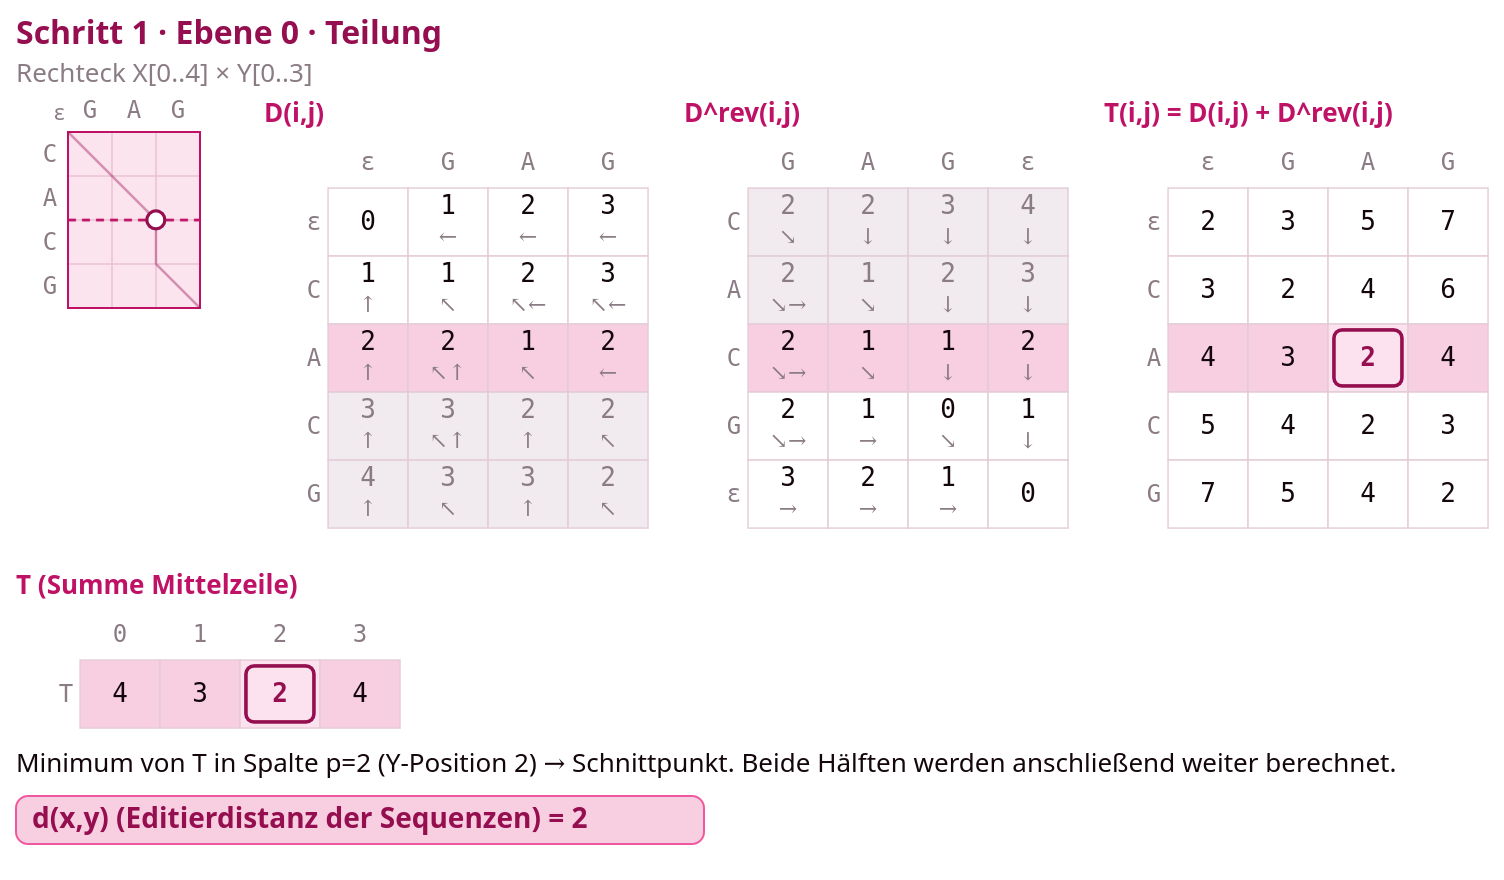
\includegraphics[width=0.6\linewidth]{images/hirschberg_CACG_GAG_schritt_1}
        \caption{Tracing}\label{fig:hirschberg_CACG_GAG_schritt_1}
    \end{figure}
\end{bsp}

\begin{bsp}
    \begin{figure}[H]
        \centering
        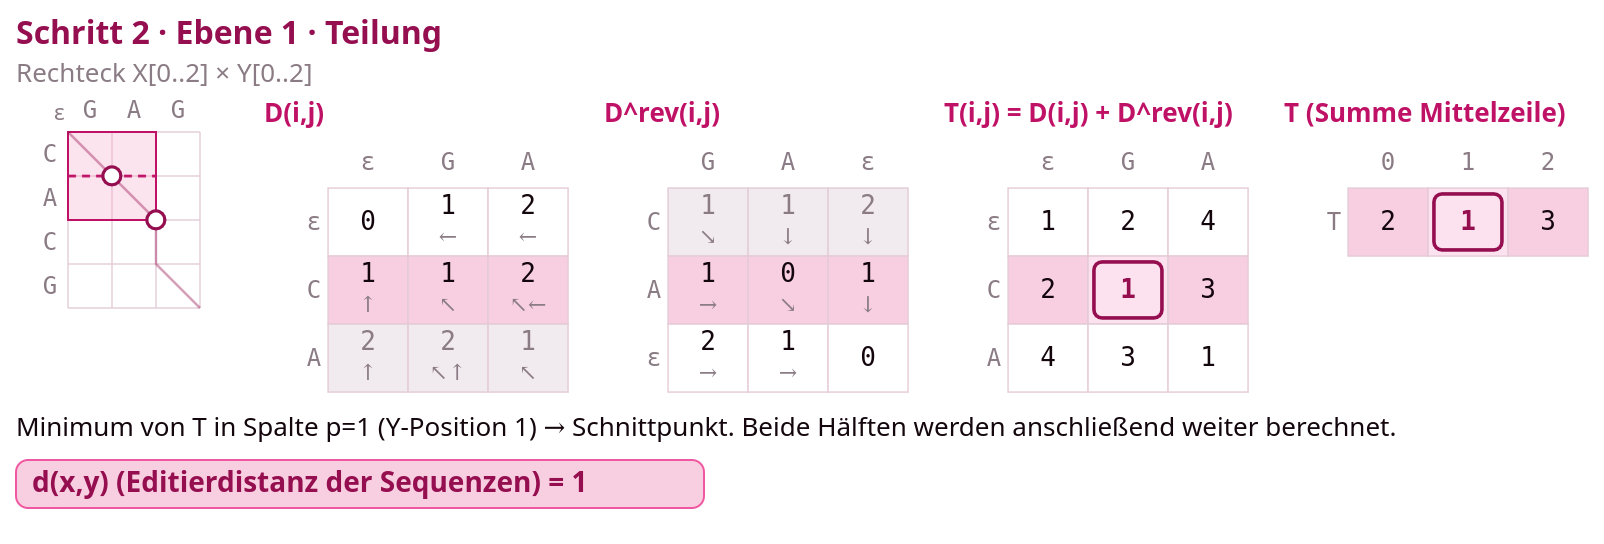
\includegraphics[width=0.6\linewidth]{images/hirschberg_CACG_GAG_schritt_2}
        \caption{Tracing}\label{fig:hirschberg_CACG_GAG_schritt_2}
    \end{figure}
\end{bsp}

\begin{bsp}
    \begin{figure}[H]
        \centering
        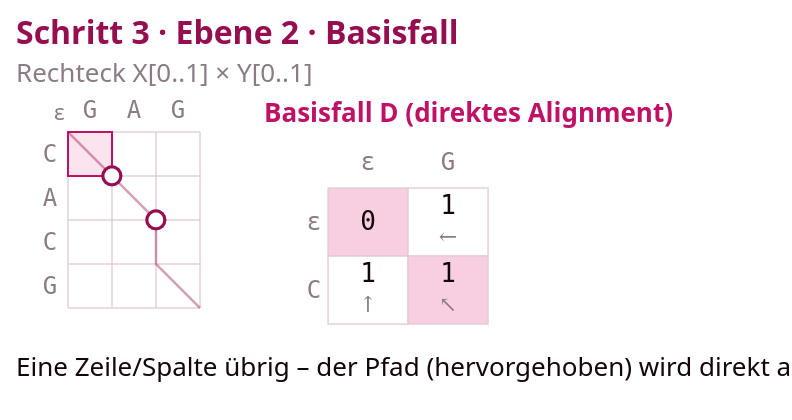
\includegraphics[width=0.6\linewidth]{images/hirschberg_CACG_GAG_schritt_3}
        \caption{Tracing}\label{fig:hirschberg_CACG_GAG_schritt_3}
    \end{figure}
\end{bsp}

\begin{bsp}
    \begin{figure}[H]
        \centering
        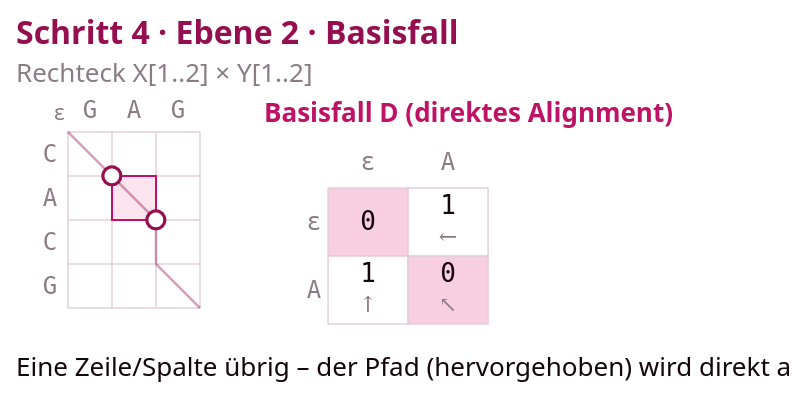
\includegraphics[width=0.6\linewidth]{images/hirschberg_CACG_GAG_schritt_4}
        \caption{Tracing}\label{fig:hirschberg_CACG_GAG_schritt_4}
    \end{figure}
\end{bsp}

\begin{bsp}
    \begin{figure}[H]
        \centering
        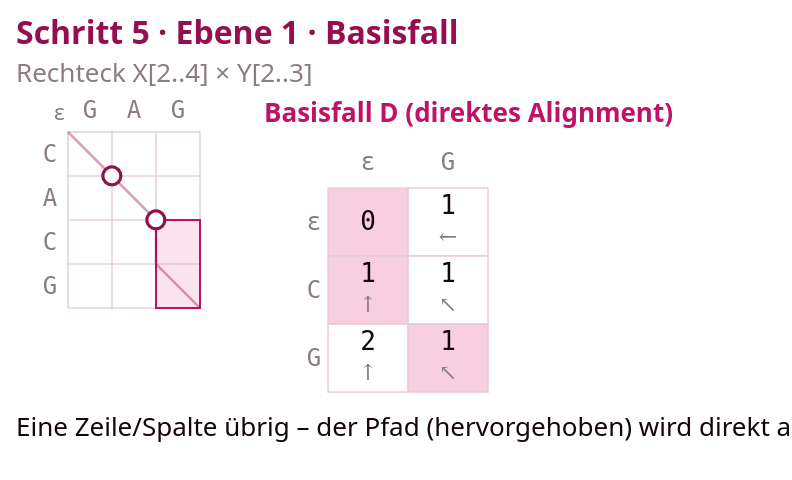
\includegraphics[width=0.6\linewidth]{images/hirschberg_CACG_GAG_schritt_5}
        \caption{Tracing}\label{fig:hirschberg_CACG_GAG_schritt_5}
    \end{figure}
\end{bsp}